%\newpage
%\vspace{-3.0pt}
\section{Problem Definition}
\label{sec:problem-definition}
%\guy{Can someone check Sections 3-4-5? Especially the formulations}


\subsection{The SER Language}

\subsubsection{Syntax}
We define the syntax of our \toolname{} language as follows: 
%of Fig.~\ref{fig:syntax}.

\[
\begin{aligned}
	\mathbf{Expression}\quad e ::= &\ 0 \mid 1 \mid 2 \mid \dots            && \text{numeric constant}\\
	&\mid \nondet                            && \text{nondeterministic\ value (0/1)}\\
%	&\mid x := e
%	&&\text{write to local variable}\\
%	&\mid x
%	&&\text{read from local variable}\\
%	&\mid X := e
%	&&\text{write to global variable}\\
%	&\mid X
%	&&\text{read from global variable}\\
	&\mid x := e \mid x                      && \text{write/read local variable}\\
	&\mid X := e \mid X                      && \text{write/read global variable}\\
	&\mid e_1 == e_2                         && \text{equality test}\\
	&\mid e_1 ; e_2                          && \text{sequencing}\\
	&\mid \ifkw(e_1)\{e_2\}\elsekw\{e_3\}    && \text{conditional}\\
	&\mid \whilekw(e_1)\{e_2\}               && \text{while loop}\\
	&\mid \yieldkw                           && \text{yield to scheduler}
	\\[0.8em]
	\mathbf{Program}\quad P_0 ::= &\ \requestkw\ name_1\{e_1\}\;\dots\;\requestkw\ name_n\{e_n\}
	&& \text{set of handlers} 
\end{aligned}
\]

%
%\[
%\begin{aligned}
%	\mathbf{Expression}\quad e ::={}&{} \\
%	&0 \mid 1 \mid 2 \mid \dots 
%	&&\grammartag{Numeric constants}\\
%	&\nondet
%	&&\grammartag{Nondeterministic value: 0 or 1}\\
%	&x := e
%	&&\grammartag{Write to local variable}\\
%	&x
%	&&\grammartag{Read from local variable}\\
%	&X := e
%	&&\grammartag{Write to global variable}\\
%	&X
%	&&\grammartag{Read from global variable}\\
%	&e_1 == e_2
%	&&\grammartag{Equality test}\\
%	&e_1 ; e_2
%	&&\grammartag{Sequencing}\\
%	&\ifkw(e_1)\{e_2\}\elsekw\{e_3\}
%	&&\grammartag{Conditional}\\
%	&\whilekw(e_1)\{e_2\}
%	&&\grammartag{While loop}\\
%	&\yieldkw
%	&&\grammartag{Yields to scheduler}\\[1em]
%	\mathbf{Program}\quad p ::={}&{} \\
%	&\requestkw\ name_1\{e_1\}
%	&&\grammartag{Set of request handlers}\\
%	&\quad\vdots\\
%	&\requestkw\ name_n\{e_n\}
%\end{aligned}
%\]
%
%%
%
%\begin{figure}[!htbp]
%    \begin{align*}
%    \mathbf{Expression}\quad e ::= &&& \\
%       | & \quad 0 \mid 1 \mid 2 \mid \ldots                                && \grammartag{Numeric constants} \\
%       | & \quad \nondet                                 && \grammartag{Nondeterministic value: 0 or 1}\\
%       | & \quad x := e                            && \grammartag{Write to local variable field} \\
%       | & \quad x                                 && \grammartag{Read from local variable field} \\
%       | & \quad X := e                            && \grammartag{Write to global  variable} \\
%       | & \quad X                                 && \grammartag{Read from global  variable} \\
%       | & \quad e_1 == e_2                        && \grammartag{Equality test} \\
%       | & \quad e_1 ; e_2                         && \grammartag{Sequencing} \\
%       | & \quad \ifkw(e_1)\{\ e_2\ \}\elsekw\{\ e_3\ \} && \grammartag{Conditional} \\
%       | & \quad \whilekw(e_1)\{\ e_2\ \}              && \grammartag{While loop} \\
%       | & \quad \yieldkw                      && \grammartag{Yields to scheduler}\\[1em]
%    \mathbf{Program}\quad p ::=
%        & \quad \requestkw\ name_1\ \{\ e_1\ \}&&\grammartag{Set of request handlers}\\[-0.5em]
%        & \quad \qquad \vdots &&\\
%        & \quad \requestkw\ name_n\ \{\ e_n\ \}\ 
%    \end{align*}
%    \caption{Syntax of expressians and programs}
%    \label{fig:syntax}
%\end{figure}
    %
%    
%
%
%
%\guy{add other rebuttal promises}
%\guy{check semantics}
%
%
% SER small-step semantics with explicit guard (congruence) rules
% Requires: \usepackage{mathtools,amssymb,mathpartir}


%Given such a \(P_0\), we write \(name_i\{e_i\}\in P_0\).
%

Given a program \(P_0\), we write \(name_i\{e_i\}\in P_0\) for each of the handlers \(name_i\{e_i\}\).
%
Our semantics is standard and fully formalized in subsection~\ref{subsec:ser-semantics}. 
 %
 In addition, arithmetic extensions are supported in the tool~\cite{ArtifactRepository} but omitted here for brevity.
%Our semantics is straightforward, and fully formalized in Appendix~\ref{appendix:ser-semantics}.
%
%Furthermore, our syntax and semantics can also be extended with \textit{arithmetic operations} (as implemented in our tool~\cite{ArtifactRepository}), but we omit them for simplicity.
%
%Furthermore, we note that our syntax and semantics can both be extended to include \textit{arithmetic operations} (as in our implementation~\cite{ArtifactRepository}); however, we omit these for simplicity. 
    
\subsubsection{Small-Step Semantics}
\label{subsec:ser-semantics}
%
%
%\subsection{Semantics}
%
The set \(\texttt{V}\) is a finite set of numeric constants; booleans use $0/1$. We respectively denote with \(\texttt{VARS}\) and \(\texttt{vars}\) the (finite) sets of global and local variables. Mappings $\rho:{\texttt{vars}}\to \texttt{V}$ and $g:{\texttt{VARS}}\to \texttt{V}$ respectively map a local or global variable to its current value in \(\texttt{V}\).
%
Configurations are denoted as $\cfg{e}{\rho}{g}$, with \(e\) being a valid \toolname{} expression. 
%
Small steps are denoted $(\step)$, while big steps are denoted $(\pstep)$, and may comprise of a sequence of small steps (denoted $\step^{*}$).
%
%program configurations $\langle g , \Pi\rangle$ with \(g\) being a global state and \(\Pi\) being set of in-flight \((e,\ell)\) pairs.
%
%We denote with \(\ell_0\) the initial local state of every packet.

\smallskip
\noindent\textit{Small step} $(\step)$.
\begin{mathpar}
	\inferrule*[right=ND-0]{ }{\cfg{\nondet}{\rho}{g} \step \cfg{0}{\rho}{g}}
	\and
	\inferrule*[right=ND-1]{ }{\cfg{\nondet}{\rho}{g} \step \cfg{1}{\rho}{g}}\\
	
	\inferrule*[right=LOCAL-READ]{\rho(x)=v\quad v\in{\texttt{V}}}{\cfg{x}{\rho}{g} \step \cfg{v}{\rho}{g}}
	\and
	\inferrule*[right=GLOBAL-READ]{g(X)=v \quad v\in{\texttt{V}}}{\cfg{X}{\rho}{g} \step \cfg{v}{\rho}{g}}\\
	
	\inferrule*[right=LOCAL-WRITE-STEP]{\cfg{e}{\rho}{g} \step \cfg{e'}{\rho'}{g'}}{\cfg{x := e}{\rho}{g} \step \cfg{x := e'}{\rho'}{g'}}
	\and
	\inferrule*[right=LOCAL-WRITE-DONE]{v\in{\texttt{V}}}{\cfg{x := v}{\rho}{g} \step \cfg{v}{\update{\rho}{x}{v}}{g}}
	
	\inferrule*[right=GLOBAL-WRITE-STEP]{\cfg{e}{\rho}{g} \step \cfg{e'}{\rho'}{g'}}{\cfg{X := e}{\rho}{g} \step \cfg{X := e'}{\rho'}{g'}}
	\and
	\inferrule*[right=GLOBAL-WRITE-DONE]{v\in{\texttt{V}}}{\cfg{X := v}{\rho}{g} \step \cfg{v}{\rho}{\update{g}{X}{v}}}
	
	\inferrule*[right=EQ-L]{\cfg{e_1}{\rho}{g} \step \cfg{e_1'}{\rho'}{g'}}{\cfg{e_1 == e_2}{\rho}{g} \step \cfg{e_1' == e_2}{\rho'}{g'}}
	\and
	\inferrule*[right=EQ-R]{\cfg{e_2}{\rho}{g} \step \cfg{e_2'}{\rho'}{g'}}{\cfg{v_1 == e_2}{\rho}{g} \step \cfg{v_1 == e_2'}{\rho'}{g'}}
	\and
	\inferrule*[right=EQ-T]{v_1=v_2\quad v_1, v_2\in{\texttt{V}}}{\cfg{v_1 == v_2}{\rho}{g} \step \cfg{1}{\rho}{g}}
	\and
	\inferrule*[right=EQ-F]{v_1\neq v_2 \quad v_1, v_2\in{\texttt{V}}}{\cfg{v_1 == v_2}{\rho}{g} \step \cfg{0}{\rho}{g}}
\end{mathpar}

\begin{mathpar}
	\inferrule*[right=SEQ-STEP]{\cfg{e_1}{\rho}{g} \step \cfg{e_1'}{\rho'}{g'}}{\cfg{e_1 ; e_2}{\rho}{g} \step \cfg{e_1' ; e_2}{\rho'}{g'}}
	\and
	\inferrule*[right=SEQ-DONE]{v\in{\texttt{V}}}{\cfg{v ; e_2}{\rho}{g} \step \cfg{e_2}{\rho}{g}}
	
	\inferrule*[right=IF-GUARD]{\cfg{e_1}{\rho}{g} \step \cfg{e_1'}{\rho'}{g'}}{\cfg{\ifkw(e_1)\{e_2\}\elsekw\{e_3\}}{\rho}{g} \step \cfg{\ifkw(e_1')\{e_2\}\elsekw\{e_3\}}{\rho'}{g'}}
	\and
	\inferrule*[right=IF-T]{ }{\cfg{\ifkw(1)\{e_2\}\elsekw\{e_3\}}{\rho}{g} \step \cfg{e_2}{\rho}{g}}
	\and
	\inferrule*[right=IF-F]{ }{\cfg{\ifkw(0)\{e_2\}\elsekw\{e_3\}}{\rho}{g} \step \cfg{e_3}{\rho}{g}}
	
	\inferrule*[right=WHILE-UNFOLD]{ }{\cfg{\whilekw(e_1)\{e_2\}}{\rho}{g}
		\step
		\cfg{\ifkw(e_1)\{\,e_2 ; \whilekw(e_1)\{e_2\}\,\}\elsekw\{0\}}{\rho}{g}}
\end{mathpar}

\noindent\textit{Big step} $(\pstep)$ and scheduling.
\begin{mathpar}
	\inferrule*[right=YIELD]{\cfg{e}{\rho}{g} \step^{*} \cfg{\yieldkw ; e'}{\rho'}{g'}}{\cfg{e}{\rho}{g} \pstep \cfg{e'}{\rho'}{g'}}
	\\
	%	\inferrule*[right=START]{\cfg{e_i}{\rho}{g}\pstep \cfg{e'_i}{\rho'}{g'} \quad name_i\{e_i\}\in P_0}{\langle \requestkw\ name_i\{e_i\}, \rho, g \rangle \pstep  \cfg{e'_i}{\rho'}{g'} }
	%	\and
	\inferrule*[right=TERMINATE]{\cfg{e}{\rho}{g} \step^{*} \cfg{v}{\rho'}{g'} \quad v\in{\texttt{V}}}{\cfg{e}{\rho}{g} \pstep \cfg{v}{\rho'}{g'}}	
\end{mathpar}



\smallskip
\noindent
\textbf{Note.}
Instead of defining a \texttt{spawn} instruction, as exists in some languages --- \toolname{} captures \textit{external} spawning via requests.
%
This setting can equivalently capture self-spawning (by using additional global variables), while translating more naturally to the networking domain --- in which threads are captured by packets sent by an external user.


\subsection{Network System}    
Motivated by software-defined networks, we present our abstract network system (NS) abstraction model. Specifically, spawning a new request corresponds to sending a \textit{packet} in the SDN domain --- with each unique \textit{packet header field} representing a request-local \toolname{} variable;
shared variables on \textit{programmable switches}, correspond to global variables, as they are seen by all the requests (packets) visiting the switch. Furthermore, we note that throughout this paper, we use the term \emph{request} to refer to a thread of a concurrent computation unit. 
%
Formally, a network system $\mathcal{N}$ is defined as an eight-tuple $(G, L, \mathit{REQ},  \mathit{RESP}, g_0, \delta, \mathit{req}, \mathit{resp})$ where:
\begin{itemize}
\item $G$ is defined as the set of reachable \textit{global network states} (for example, the values of switch variables)

\item $L$ is defined as the set of reachable \textit{local packet states} (e.g., the values of packet header variables)

\item $\mathit{REQ}$ is a finite set of \textit{request label strings} (with each request label denoted as {\color{ForestGreen}$\blacklozenge_\text{req}$})

\item $\mathit{RESP}$ is a finite set of \textit{response label strings} (with each response label denoted as {\color{red}$\blacklozenge_\text{resp}$})

\item $g_0 \in G$ is the networks system's \textit{initial global state}

\item $\mathit{req} \subseteq \mathit{REQ} \times  L$ is a mapping from each request label to its corresponding (initial) local state; we note that this represents an external user that spawns a packet as part of the system interface

\item $\mathit{resp} \subseteq L \times \mathit{RESP}$ is a mapping from a final local state to the corresponding response; we note that this represents a packet that exits the network and returns a computation to the user

\item $\delta \subseteq  (L \times G) \times ( L \times G)$ is a mapping that corresponds to the atomic execution steps updating both (request) local and (system) global state; intuitively, this represents a single hop of a single packet in the network
%(and the corresponding SER expressions); as based on SER's small-step semantics
\end{itemize}

%\todo{new start}
%We refer to our transition rules in Fig.~\ref{fig:code2ExampleNS}.

%\smallskip
\noindent
\textbf{Request and response.}
A \emph{request} label ${\color{ForestGreen}\blacklozenge_\text{req}}\in\mathit{REQ}$ spawns a new request thread (i.e., a packet) which is computed concurrently based on the program; a \emph{response} label ${\color{red}\blacklozenge_\text{resp}}\in\mathit{RESP}$ is the returned value of this computation. Together, the $({\color{ForestGreen}\blacklozenge_\text{req}},{\color{red}\blacklozenge_\text{resp}})$ pair captures the observable input/output behavior of a single with regard to a single request from a single concurrent execution of the network system.



\smallskip
\noindent
\textbf{States.}
A \emph{network state} is a triple $(g,\mathcal{R},\mathcal{Z})$ in which $g \in G$ is the current global state of the network,
$\mathcal{R} \in \mathrm{Multiset}(L \times \mathit{REQ})$ is a multiset of requests threads that are currently \textit{in-flight}, i.e., local assignments of each thread in the current timestep, coupled with the original request label that spawned it; and $\mathcal{Z} \in \mathrm{Multiset}(\mathit{REQ} \times \mathit{RESP})$ is a multiset of request/response pairs that have terminated.
%
We denote with $\uplus$ the multiset union.
%
Furthermore, the initial global state of the network system is the triple $(g_0, \varnothing, \varnothing)$.




% Non-figure version of the state-transition rules (caption text inlined)
%\renewcommand{\arraystretch}{1.6}
%\medskip
\smallskip
\noindent
\textbf{Transition rules.}
The network system semantics define that a transition $\longrightarrow$ can either (1) spawn a new request; (2) advances one request via the $\delta$ mapping; or (3) return a response to an in-flight request. When no further steps remain, then $\mathcal{Z}$ is the final multiset of request/response pairs as induced by the interleaving of the network system's execution.




%\noindent\textbf{States and transitions.}
%A (global) \emph{network state} is a triple $(g,\mathcal{R},M)$ where
%$g \in G$ is the current global state,
%$\mathcal{R} \in \mathrm{Multiset}(L \times \mathit{REQ})$ is a multiset of in-flight requests (threads),
%and $M \in \mathrm{Multiset}(\mathit{REQ} \times \mathit{RESP})$ is a multiset of completed request/response pairs.
%%
%The initial state is $(g_0, \varnothing, \varnothing)$.


%\smallskip
%\noindent\textbf{Initial state.} $(g_0, \varnothing, \varnothing)$.

%\smallskip
%\noindent\textbf{Transition rules.}
\[
\text{(New Request)}\quad
\infer{({\color{ForestGreen}\blacklozenge_\text{req}},\ell)\in\mathit{req}}
{(g,\mathcal{R},\mathcal{Z}) \rightarrow (g,\; \mathcal{R}\uplus\{(\ell,{\color{ForestGreen}\blacklozenge_\text{req}})\},\; \mathcal{Z})}
\]
\[
\text{(Processing Step)}\quad
\infer{((\ell, g),(\ell', g'))\in\delta}
{(g,\; \mathcal{R}\uplus\{(\ell,{\color{ForestGreen}\blacklozenge_\text{req}})\},\; \mathcal{Z})
	\rightarrow
	(g',\; \mathcal{R}\uplus\{(\ell',{\color{ForestGreen}\blacklozenge_\text{req}})\},\; \mathcal{Z})}
\]
\[
\text{(Response)}\quad
\infer{(\ell,{\color{red}\blacklozenge_\text{resp}})\in\mathit{resp}}
{(g,\; \mathcal{R}\uplus\{(\ell,{\color{ForestGreen}\blacklozenge_\text{req}})\},\; \mathcal{Z})
	\rightarrow
	(g,\; \mathcal{R},\; \mathcal{Z} \uplus \{({\color{ForestGreen}\blacklozenge_\text{req}},{\color{red}\blacklozenge_\text{resp}})\})}
\]


\smallskip
\noindent
\textbf{Serializability.}
We define an \textit{interleaved run} as the complete execution 
\((g_0,\varnothing,\varnothing)\!\to^*\!(g_n,\varnothing,\mathcal{Z})\):
\[
(g_0,\varnothing,\varnothing) \;\to\; (g_1,\mathcal{R}_1,\mathcal{Z}_1) \;\to\; \cdots \;\to\; 
%(g_{n-1},\mathcal{R}_{n-1},\mathcal{Z}_{n-1}) \;\to\; 
(g_n,\mathcal{R}_{n},\mathcal{Z}_{n}),
\quad
\text{with } \mathcal{R}_{n}=\varnothing,\mathcal{Z}_n=\mathcal{Z}.
 %\varnothing,Z
\]
We says that an interleaved run is \textit{serial} if it adheres to the constraints that each $\mathcal{R}_i$ has \textit{at most} a single request in-flight.
%
Intuitively, serial runs process at every time-step a single request until completion.
%	,
%	whereas \emph{interleaved} runs may have multiple requests in flight at once.
	%
	%
	Given a network system \(\mathcal{S}\), we respectively denote by \(\mathsf{Int}(\mathcal{S})\) and \(\mathsf{Ser}(\mathcal{S})\) the (infinite) sets of request/response multisets, as induced by the interleaved and serial runs of \(\mathcal{S}\) accordingly:
%
\[
\mathsf{Int}(\mathcal{S})=\{\,\mathcal{Z}\mid \exists\text{ \textit{interleaved} run }(g_0,\varnothing,\varnothing)\rightarrow^{*}(g_n,\varnothing,\mathcal{Z})\,\},
\]
\[
\mathsf{Ser}(\mathcal{S})=\{\,\mathcal{Z}\mid \exists\text{ \textit{serial} run }(g_0,\varnothing,\varnothing)\rightarrow^{*}(g_n,\varnothing,\mathcal{Z})\,\}\subseteq \mathsf{Int}(\mathcal{S}).
\]
%\todo{old}
%\[
%\mathrm{Int}(\mathcal{N})
%= \bigl\{\, \mathcal{Z} \in \mathrm{Multiset}(\mathit{REQ}\times \mathit{RESP})
%\;\big|\; \exists\ \text{\textit{interleaved} run } (g_0,\varnothing,\varnothing)\rightarrow^{*}(g_n,\varnothing,\mathcal{Z}) \,\bigr\}
%\]
%%
%\[
%\mathrm{Ser}(\mathcal{N})
%= \bigl\{\, \mathcal{Z} \in \mathrm{Multiset}(\mathit{REQ}\times \mathit{RESP})
%\;\big|\; \exists\ \text{\textit{serial} run } (g_0,\varnothing,\varnothing)\rightarrow^{*}(g_n,\varnothing,\mathcal{Z}) \,\bigr\}.
%\]

The network system $\mathcal{S}$ is said to be \emph{serializable} if and only if \(\mathsf{Int}(\mathcal{S})=\mathsf{Ser}(\mathcal{S})\). Differently put, every multiset of request/response pairs that can be induced by an interleaved execution can also be induced by a serial one.


%
%\todo{old}
%\smallskip
%\noindent
%\textbf{Serializability.}
%We define an \textit{interleaving run} of the network system as a complete execution (also denoted \((g_0,\varnothing,\varnothing)\rightarrow^{*}(g_n,\varnothing,Z)\)):
%%\noindent\textbf{Complete runs.}
%\[
%(g_0,\varnothing,\varnothing) \rightarrow (g_1,\mathcal{R}_1,Z_1)
%\rightarrow \cdots \rightarrow (g_n,\mathcal{R}_{n-1},Z_{n-1}) \rightarrow (g_n,\varnothing,Z_n).
%\]
%
%\noindent
%%A full run is also denoted \((g_0,\varnothing,\varnothing)\rightarrow^{*}(g_n,\varnothing,Z)\), and is called an \textit{interleaved} run if the $\mathcal{R}_i$ may contain multiple requests and $\mathcal{R}_n=\varnothing$.
%%
%An interleaved run is said to be \textit{serial} if each $\mathcal{R}_i$ has \textit{at most} one request, and $\mathcal{R}_n=\varnothing$.
%%
%Intuitively, \textit{serial} runs have at most one request in flight at any time,
%whereas \emph{interleaved} runs may have multiple requests in flight at once.
%%
%For a network system \(\mathcal{N}\), we define \(\mathrm{Int}(\mathcal{N})\) and \(\mathrm{Ser}(\mathcal{N})\) to  represent the set of all multisets of request/response pairs, for interleaving and serializable runs respectively:
%
%\[
%\mathrm{Int}(\mathcal{N})
%= \bigl\{\, Z \in \mathrm{Multiset}(\mathit{REQ}\times \mathit{RESP})
%\;\big|\; \exists\ \text{\textit{interleaved} run } (g_0,\varnothing,\varnothing)\rightarrow^{*}(g_n,\varnothing,Z) \,\bigr\}
%\]
%\[
%\mathrm{Ser}(\mathcal{N})
%= \bigl\{\, Z \in \mathrm{Multiset}(\mathit{REQ}\times \mathit{RESP})
%\;\big|\; \exists\ \text{\textit{serial} run } (g_0,\varnothing,\varnothing)\rightarrow^{*}(g_n,\varnothing,Z) \,\bigr\}.
%\]
%
%
%
%A network system $\mathcal{N}$ is \emph{serializable} if $\text{Int}(\mathcal{N}) = \text{Ser}(\mathcal{N})$, i.e., every multiset of request/response pairs attainable through an interleaved execution can also be attained through a serial one.

\subsection{From SER Programs to Network Systems}
\label{subsec:SerToNsTranslation}
%
The network system abstraction does not merely encode concurrent behaviors in the SDN domain, but also can be naturally translated from \toolname{} programs. 
More formally, given an input \toolname{} program \(P_0\) with global variables (\texttt{VARS}), local variables (\texttt{vars}), mappings \(g,\rho\) from these global/local assignments to a finite number of elements from a value set \texttt{V} --- we define the initial global/local states, $g_0$ and $\rho_0$, which respectively assign $0$ to all global and local variables. 
Building on the small-step semantics ($\pstep$, defined in full in subsec.~\ref{subsec:ser-semantics}), we define the network system $(G, L, \mathit{REQ}, \mathit{RESP}, g_0, \delta, \mathit{req}, \mathit{resp})$ as follows:

%\todo{old}
%The NS abstraction is useful beyond its capability to capture concurrent behaviors in software-defined networks.
%%
%Specifically, another advantage is the natural translation from  \toolname{} programs to their corresponding NS.
%%, as we demonstrate next.
%%
%%
%%\smallskip
%%\noindent
%Given a \toolname{} program \(P_0\) with: (i) local variables (\texttt{vars}); (ii) global variables (\texttt{VARS}); (iii) mappings \(\rho\) and (iv) \(g\) from local/global variables to (v) a finite set of values \texttt{V}.
%%
%We define the initial (local) state $\rho_0$ and the initial (global) state $g_0$ to assign $0$ to all variables, respectively.
%%
%Furthermore, given the small steps semantics ($\pstep$ defined in App.~\ref{appendix:ser-semantics}), we construct the following NS $(G, L, \mathit{REQ},  \mathit{RESP}, g_0, \delta, \mathit{req}, \mathit{resp})$:

\[
\begin{aligned}
	G \;&=\; \{\, g : \texttt{VARS}\!\to\! \texttt{V} \,\},\\[0.3ex]
	L \;&=\; \bigl\{\, (e,\rho)\ \bigm|\ \rho:\texttt{vars}\!\to\! \texttt{V},\ \exists\,name_i\{e_i\}\!\in\! P_0\ \text{s.t.} \\[-0.2ex]
	&\qquad\quad\qquad\quad e=e_i \text{ or } e \text{ is a suffix of } e_i \text{ starting after a } \yieldkw \text{ statement}\,\bigr\},\\[0.3ex]
	REQ \;&=\; \{\, name_i \mid name_i\{e_i\}\!\in\! P_0 \,\},\quad RESP \;=\; \texttt{V},\\[0.3ex]
	req \;&=\; \{\, (r,\ell) \mid r=name_i\!\in\!REQ,\ name_i\{e_i\}\!\in\! P_0,\ \ell=(e_i,\rho_0)\!\in\!L\},\\[0.3ex]
	resp \;&=\; \{\, (\ell',r') \mid \exists v\!\in\!\texttt{V}.\ \ell'=(v,\rho')\!\in\!L,\ r'=v\!\in\!RESP \,\},\\[0.3ex]
	\delta \;&=\; \bigl\{\, ((e,\rho),g)\!\to\!((e',\rho'),g') \ \bigm|\ (e,\rho),(e',\rho')\!\in\!L,\ g,g'\!\in\!G,\ 
	\cfg{e}{\rho}{g} \pstep \cfg{e'}{\rho'}{g'} \,\bigr\}.
\end{aligned}
\]


%
%\begin{itemize}
%	\item The set of global states include all mappings from global variables to values:
%	\[
%	G = \{\, g \mid g : \text{VARS} \to V \,\}.
%	\]
%	
%	\item The set of local states include a pair of the local variable assignments coupled with the remaining \toolname{} program to execute, i.e., a sequence of expressions until: (i) the subsequent \(\yieldkw\); or (ii) termination
%	\[
%	L = \{\, (r,\rho) \mid \exists \rho : \text{vars} \to V \ \exists \, name_i\{e_i\} \in P_0 \ \exists k \ge 0 \,.\, (e_k';\yieldkw)^k ; e = e_i \in P_0 \,\}.
%	\]
%
%	
%	\item The set of requests are the handlers of the \toolname{} program:
%	\[
%	REQ = \{\, name_i \mid name_i\{e_i\} \in P_0 \,\}.
%	\]
%	
%	\item The set of responses include all possible numerical constants:
%	\[
%	RESP = V.
%	\]
%	
%	\item The request relation maps every request to a local state with the corresponding request handler and the initial local assignment:
%	\[
%	req = \{\, (r,\ell) \mid r = name_i \in REQ, \, \ell = (e_i,\rho_0) \in L \,\}.
%	\]
%	
%	\item The response relation maps the computed constant (attained prior to termination) with the corresponding response:
%	\[
%	resp = \{\, (\ell',r') \mid \exists v \in V \,.\, \ell' = (v',\rho') \in L, \, r' \in RESP \,\}.
%	\]
%	
%	\item The transition relation, defined according to the \toolname{} semantics:
%	\[
%	\delta = \bigl\{ \, 
%	(((e,\rho),g),((e',\rho'),g')) \,\bigm|\, 
%	(e,\rho),(e',\rho') \in L, \ g,g' \in G, \ 
%	\cfg{e}{\rho}{g} \pstep \cfg{v}{\rho'}{g'} 
%	\,\bigr\}.
%	\]
%\end{itemize}
%



% $\mathit{req} \subseteq \mathit{REQ} \times  L$ maps each request type to its corresponding local state
%initial SER expression and  local state
%
% $\mathit{resp} \subseteq L \times \mathit{RESP}$ maps final SER expressions and local states to response types
%
% $\delta \subseteq  (L \times G) \times ( L \times G)$ defines atomic execution steps that update both global and local state 
%(and the corresponding SER expressions); as based on SER's small-step semantics



%\smallskip
%\noindent
%\textbf{Assumptions.}
%%
%In addition to the assumption that the request and response sets are finite, we also assume that a program has a \textit{finite number of reachable states}. 
%%
%These states are enumerated when converting a \toolname{} program to a Network System. 
%%
%For convenience, the input program may be written with unbounded values as long as only a finite number are actually reached. 
%%
%If the program can reach an infinite number of states, then this initial Network System conversion times out. 
%
%If the input program is written with restricted syntax shown in the SER syntax, then the SER \(\step\) NS conversion always terminates. 


%\subsection{NS Example: Non-Serializability }
%\label{sec:ns-non-serializable}
%\medskip
%\noindent
%\textbf{Example: \toolname{} to NS.}
%
\begin{tcolorbox}[colback=black!5!white, colframe=black, boxrule=1pt]
\textbf{Example.}
We demonstrate the network system corresponding to the non-serializable \toolname{} program in Listing~\ref{lst:MotivatingExample2NonSer}:
%
\begin{itemize}
\item 
We define the set $G$ as $G=\{[\texttt{X=0}], [\texttt{X=1}]\}$.

\item 
We define the initial global state as $g_0 = [\texttt{X=0}]$.

\item 
We define the set $L$ as all the \textit{reachable} local states, i.e., pairs of assignments (in this case, $[\texttt{y=0}], [\texttt{y=1}]$) that are coupled with all reachable \toolname{} programs, i.e., continuations of a program at a given execution point.
%~\footnote{
%These are continuations of a \toolname{} program at a point of execution. Concretely, this can mean either (i) the suffix of the program when it is first initialized (the part that has not yet executed); or (ii) the continuation of the program after a \(\yieldkw\) statement, where execution may later resume.}.
For instance, the reachable programs for Listing~\ref{lst:MotivatingExample2NonSer} are depicted in the code snippets of Fig.~\ref{fig:code2ExampleNS}. 


\item 
We define the set of requests as $REQ = \{{\color{ForestGreen}\blacklozenge_\text{main}}\}$.

\item 
We define the set of responses as $RESP = \{{\color{red}\blacklozenge_0},{\color{red}\blacklozenge_1}\}$.

\item
Finally, we define the \(\delta\) function to capture the program behavior. This is depicted in Fig.~\ref{fig:code2ExampleNSSecondPart}.


\end{itemize}


Fig.~\ref{fig:code2ExampleNS} presents the explicit network system that
resulted from this translation. This NS can also be seen as a mapping from request labels ({\color{ForestGreen}$\blacklozenge_\text{main}$}) to response labels ({\color{red}$\blacklozenge_0$}, {\color{red}$\blacklozenge_1$}).
%
%We note that, for simplicity, we depict only \textit{reachable} states.
%
\end{tcolorbox}


\begin{figure}[!htbp]
	\centering
	%–––– Network system diagram ––––
	% \includegraphics[width=\textwidth]{plots/code_2_NS.png}\\[1ex]
	
	%–––– req, resp, and δ definitions ––––
	\[
	\begin{array}{@{}r@{\;}l}
		req \coloneq & 
		\big\{
		\big[
		\begin{array}{c c c}
			\begin{tikzpicture}[baseline=(textnode.base)]
				\node[
				draw=black,
				line width=0.8pt,
				fill=ForestGreen!20,
				text=black,
				diamond,
				aspect=2,
				inner sep=2pt,
				scale=0.7
				] (textnode) {\texttt{main}};
			\end{tikzpicture}
			&\!\!\rightarrow\!\!&
			\begin{array}{c}
				\begin{tikzpicture}[baseline=(ybox.base)]
					\node[
					draw=black,
					line width=0.8pt,
					fill=brightyellow,
					text=black,
					rectangle,
					rounded corners=1pt,
					inner sep=2pt
					] (ybox) {\texttt{y=0}};
				\end{tikzpicture}\vspace{-2pt}
				\\
				\begin{minipage}{0.20\linewidth}
					\begin{lstlisting}[language=CustomPseudoCode,numbers=none,basicstyle=\tiny\ttfamily]
X := 1 
yield 
y := X
X := 0
return y
					\end{lstlisting}
				\end{minipage}
			\end{array}
		\end{array}
		\big]
		\big\}
		\\[2em]
		resp \coloneq &
		\big\{
		\big[
		\begin{array}{c c c}
			\begin{array}{c}
				\begin{tikzpicture}[baseline=(ybox.base)]
					\node[
					draw=black,
					line width=0.8pt,
					fill=brightyellow,
					text=black,
					rectangle,
					rounded corners=1pt,
					inner sep=2pt
					] (ybox) {\texttt{y=0}};
				\end{tikzpicture}\vspace{-2pt}
				\\
				\begin{minipage}{0.11\linewidth}
					\begin{lstlisting}[language=CustomPseudoCode,numbers=none,basicstyle=\tiny\ttfamily]
return y
					\end{lstlisting}
				\end{minipage}
			\end{array}
			&\!\!\rightarrow\!\!&
			\begin{tikzpicture}[baseline=(textnode.base),scale=0.7]
				\node[
				draw=black,
				line width=0.8pt,
				fill=RedViolet!20,
				text=black,
				diamond,
				aspect=2,
				inner sep=2pt,
				font=\small
				] (textnode) {\texttt{0}};
			\end{tikzpicture}
		\end{array}
		\big]\,{},
		\big[
		\begin{array}{c c c}
			\begin{array}{c}
				\begin{tikzpicture}[baseline=(ybox.base)]
					\node[
					draw=black,
					line width=0.8pt,
					fill=brightyellow,
					text=black,
					rectangle,
					rounded corners=1pt,
					inner sep=2pt
					] (ybox) {\texttt{y=1}};
				\end{tikzpicture}\vspace{-2pt}
				\\
				\begin{minipage}{0.11\linewidth}
					\begin{lstlisting}[language=CustomPseudoCode,numbers=none,basicstyle=\tiny\ttfamily]
return y
					\end{lstlisting}
				\end{minipage}
			\end{array}
			&\!\!\rightarrow\!\!&
			\begin{tikzpicture}[baseline=(textnode.base),scale=0.7]
				\node[
				draw=black,
				line width=0.8pt,
				fill=RedViolet!20,
				text=black,
				diamond,
				aspect=2,
				inner sep=2pt,
				font=\small
				] (textnode) {\texttt{1}};
			\end{tikzpicture}
		\end{array}
		\big]
		\big\}
		\\[2em]
		\delta \coloneq & 
		\big\{\big[(
		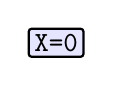
\begin{tikzpicture}[baseline=(ybox.base)]
			\node[
			draw=black,
			line width=0.8pt,
			fill=blue!10,
			text=black,
			rectangle,
			rounded corners=1pt,
			inner sep=2pt
			] (ybox) {\texttt{X=0}};
		\end{tikzpicture}\,{},
		\begin{array}{c}
			\begin{tikzpicture}[baseline=(ybox.base)]
				\node[
				draw=black,
				line width=0.8pt,
				fill=brightyellow,
				text=black,
				rectangle,
				rounded corners=1pt,
				inner sep=2pt
				] (ybox) {\texttt{y=0}};
			\end{tikzpicture}\vspace{-2pt}
			\\
			\begin{minipage}{0.14\linewidth}
				\begin{lstlisting}[language=CustomPseudoCode,numbers=none,basicstyle=\tiny\ttfamily]
X := 1
yield
y := X
X := 0
return y
				\end{lstlisting}
			\end{minipage}
		\end{array}
		)
		\;\rightarrow\;
		(
		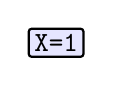
\begin{tikzpicture}[baseline=(ybox.base)]
			\node[
			draw=black,
			line width=0.8pt,
			fill=blue!10,
			text=black,
			rectangle,
			rounded corners=1pt,
			inner sep=2pt
			] (ybox) {\texttt{X=1}};
		\end{tikzpicture}\,{},
		\begin{array}{c}
			\begin{tikzpicture}[baseline=(ybox.base)]
				\node[
				draw=black,
				line width=0.8pt,
				fill=brightyellow,
				text=black,
				rectangle,
				rounded corners=1pt,
				inner sep=2pt
				] (ybox) {\texttt{y=0}};
			\end{tikzpicture}\vspace{-2pt}
			\\
			\begin{minipage}{0.14\linewidth}
				\begin{lstlisting}[language=CustomPseudoCode,numbers=none,basicstyle=\tiny\ttfamily]
y := X
X := 0
return y
				\end{lstlisting}
			\end{minipage}
		\end{array}
		)
		\big],
		\\[0.5em]
		& \phantom{\big\{}
		\big[(
		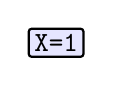
\begin{tikzpicture}[baseline=(ybox.base)]
			\node[
			draw=black,
			line width=0.8pt,
			fill=blue!10,
			text=black,
			rectangle,
			rounded corners=1pt,
			inner sep=2pt
			] (ybox) {\texttt{X=1}};
		\end{tikzpicture}\,{},
		\begin{array}{c}
			\begin{tikzpicture}[baseline=(ybox.base)]
				\node[
				draw=black,
				line width=0.8pt,
				fill=brightyellow,
				text=black,
				rectangle,
				rounded corners=1pt,
				inner sep=2pt
				] (ybox) {\texttt{y=0}};
			\end{tikzpicture}\vspace{-2pt}
			\\
			\begin{minipage}{0.14\linewidth}
				\begin{lstlisting}[language=CustomPseudoCode,numbers=none,basicstyle=\tiny\ttfamily]
y := X
X := 0
return y
				\end{lstlisting}
			\end{minipage}
		\end{array}
		)
		\;\rightarrow\;
		(
		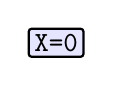
\begin{tikzpicture}[baseline=(ybox.base)]
			\node[
			draw=black,
			line width=0.8pt,
			fill=blue!10,
			text=black,
			rectangle,
			rounded corners=1pt,
			inner sep=2pt
			] (ybox) {\texttt{X=0}};
		\end{tikzpicture}\,{},
		\begin{array}{c}
			\begin{tikzpicture}[baseline=(ybox.base)]
				\node[
				draw=black,
				line width=0.8pt,
				fill=brightyellow,
				text=black,
				rectangle,
				rounded corners=1pt,
				inner sep=2pt
				] (ybox) {\texttt{y=1}};
			\end{tikzpicture}
			\vspace{-2pt}
			\\
			\begin{minipage}{0.11\linewidth}
				\begin{lstlisting}[language=CustomPseudoCode,numbers=none,basicstyle=\tiny\ttfamily]
return y
				\end{lstlisting}
			\end{minipage}
		\end{array}
		)
		\big],
		\ldots
		\big\}
	\end{array}
	\]
	\caption{The \(\delta\) transition function, and the \(req\) and \(resp\) mappings for the program in Listing~\ref{lst:MotivatingExample2NonSer}.}
	\label{fig:code2ExampleNSSecondPart}
\end{figure}



\begin{figure}[!htbp]
	\centering
	%–––– Network system diagram ––––
	% \includegraphics[width=\textwidth]{plots/code_2_NS.png}\\[1ex]

	\begin{tikzpicture}[
		node distance=1.5cm and 2.5cm,
		>=stealth,
		thick,
		every node/.style={font=\small}
	]
	  % [main request] -> [y=0][full program below that] ---[X=1 -> X=1][X=0 -> X=1 below that]--->[y=0][rest of program below that]
	  %   (first outgoing edge of last node on previous line)
      %   --[X=0 -> X=0]-->[y=0][empty program below that] ---> [0 response]
	  %   (second outgoing edge)
	  %   --[X=1 -> X=0]-->[y=1][empty program below that] ---> [1 response]
	  
	  % Main request node
	  \node[
		draw=black,
		line width=0.8pt,
		fill=ForestGreen!20,
		text=black,
		diamond,
		aspect=2,
		inner sep=2pt,
		scale=0.7
	  ] (main) {\texttt{main}};
	  
	  % First state node with full program
	  \node[right=0.7cm of main, align=center] (state1) {
		\begin{tikzpicture}[baseline=(ybox.base)]
			\node[
			draw=black,
			line width=0.8pt,
			fill=brightyellow,
			text=black,
			rectangle,
			rounded corners=1pt,
			inner sep=2pt
			] (ybox) {\texttt{y=0}};
		\end{tikzpicture}\\[-2.5pt]
		\begin{minipage}{1.0cm}
			\begin{lstlisting}[language=CustomPseudoCode,numbers=none,basicstyle=\tiny\ttfamily]
X := 1
yield
y := X
X := 0
return y
			\end{lstlisting}
		\end{minipage}
	  };
	  
	  % Second state node with rest of program
	  \node[right=of state1, align=center] (state2) {
		\begin{tikzpicture}[baseline=(ybox.base)]
			\node[
			draw=black,
			line width=0.8pt,
			fill=brightyellow,
			text=black,
			rectangle,
			rounded corners=1pt,
			inner sep=2pt
			] (ybox) {\texttt{y=0}};
		\end{tikzpicture}\\[-2.5pt]
		\begin{minipage}{1.0cm}
			\begin{lstlisting}[language=CustomPseudoCode,numbers=none,basicstyle=\tiny\ttfamily]
y := X
X := 0
return y
			\end{lstlisting}
		\end{minipage}
	  };
	  
	  % Final state y=0 with empty program
	  \node[above right=-0.5cm and 2.2cm of state2, align=center] (state3) {
		\begin{tikzpicture}[baseline=(ybox.base)]
			\node[
			draw=black,
			line width=0.8pt,
			fill=brightyellow,
			text=black,
			rectangle,
			rounded corners=1pt,
			inner sep=2pt
			] (ybox) {\texttt{y=0}};
		\end{tikzpicture}\\[-2.5pt]
		\begin{minipage}{1.0cm}
			\begin{lstlisting}[language=CustomPseudoCode,numbers=none,basicstyle=\tiny\ttfamily]
return y
			\end{lstlisting}
		\end{minipage}
	  };
	  
	  % Final state y=1 with empty program
	  \node[below right=-0.2cm and 2.2cm of state2, align=center] (state4) {
		\begin{tikzpicture}[baseline=(ybox.base)]
			\node[
			draw=black,
			line width=0.8pt,
			fill=brightyellow,
			text=black,
			rectangle,
			rounded corners=1pt,
			inner sep=2pt
			] (ybox) {\texttt{y=1}};
		\end{tikzpicture}\\[-2.5pt]
		\begin{minipage}{1.0cm}
			\begin{lstlisting}[language=CustomPseudoCode,numbers=none,basicstyle=\tiny\ttfamily]
return y
			\end{lstlisting}
		\end{minipage}
	  };
	  
	  % Response 0
	  \node[
		right=0.6cm of state3,
		draw=black,
		line width=0.8pt,
		fill=RedViolet!20,
		text=black,
		diamond,
		aspect=2,
		inner sep=2pt,
		scale=0.7,
		font=\Large
	  ] (resp0) {\texttt{0}};
	  
	  % Response 1
	  \node[
		right=0.6cm of state4,
		draw=black,
		line width=0.8pt,
		fill=RedViolet!20,
		text=black,
		diamond,
		aspect=2,
		inner sep=2pt,
		scale=0.7,
		font=\Large
	  ] (resp1) {\texttt{1}};
	  
	  % Arrows
	  \draw[->] (main) -- (state1);
	  
	  % Transition labels for state1 to state2
	  \draw[->] (state1) -- node[above] {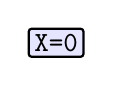
\begin{tikzpicture}[baseline=(a.base)]\node[draw=black,line width=0.8pt,fill=blue!10,rectangle,rounded corners=1pt,inner sep=2pt] (a) {\texttt{X=0}};\end{tikzpicture} $\to$ 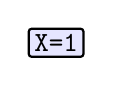
\begin{tikzpicture}[baseline=(b.base)]\node[draw=black,line width=0.8pt,fill=blue!10,rectangle,rounded corners=1pt,inner sep=2pt] (b) {\texttt{X=1}};\end{tikzpicture}} node[below] {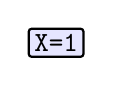
\begin{tikzpicture}[baseline=(c.base)]\node[draw=black,line width=0.8pt,fill=blue!10,rectangle,rounded corners=1pt,inner sep=2pt] (c) {\texttt{X=1}};\end{tikzpicture} $\to$ 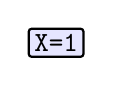
\begin{tikzpicture}[baseline=(d.base)]\node[draw=black,line width=0.8pt,fill=blue!10,rectangle,rounded corners=1pt,inner sep=2pt] (d) {\texttt{X=1}};\end{tikzpicture}} (state2);
	  
	  % From state2 to final states
	  \draw[->] ([yshift=4pt]state2.east) to[out=50,in=180] node[above, sloped] {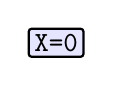
\begin{tikzpicture}[baseline=(a.base)]\node[draw=black,line width=0.8pt,fill=blue!10,rectangle,rounded corners=1pt,inner sep=2pt] (a) {\texttt{X=0}};\end{tikzpicture} $\to$ 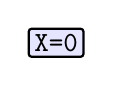
\begin{tikzpicture}[baseline=(b.base)]\node[draw=black,line width=0.8pt,fill=blue!10,rectangle,rounded corners=1pt,inner sep=2pt] (b) {\texttt{X=0}};\end{tikzpicture}} (state3.west);
	  \draw[->] ([yshift=-16pt]state2.east) to[out=-50,in=180] node[below, sloped] {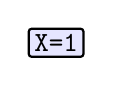
\begin{tikzpicture}[baseline=(a.base)]\node[draw=black,line width=0.8pt,fill=blue!10,rectangle,rounded corners=1pt,inner sep=2pt] (a) {\texttt{X=1}};\end{tikzpicture} $\to$ 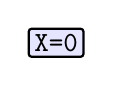
\begin{tikzpicture}[baseline=(b.base)]\node[draw=black,line width=0.8pt,fill=blue!10,rectangle,rounded corners=1pt,inner sep=2pt] (b) {\texttt{X=0}};\end{tikzpicture}} (state4.west);
	  
	  % To responses
	  \draw[->] (state3) -- (resp0);
	  \draw[->] (state4) -- (resp1);
	  
	\end{tikzpicture}
	\caption{
	The network system from the translated \toolname{} program in Listing~\ref{lst:MotivatingExample2NonSer}. 
	Local states (depicted by yellow rectangles \fcolorbox{black}{brightyellow}{\rule{0pt}{7pt}\rule{7pt}{0pt}}) present the request-local variable assignments coupled with the remaining code; edges indicate transitions of global states  (depicted by blue rectangles \fcolorbox{black}{blue!10}{\rule{0pt}{7pt}\rule{7pt}{0pt}}). 
	The request and response labels are denoted by {\color{ForestGreen!20}$\blacklozenge$} (green) and
		{\color{RedViolet!20}$\blacklozenge$} (red) diamonds, respectively.
		From left to right: a request label ${\color{ForestGreen}\blacklozenge_{\text{main}}}$ spawns a new request with initial local variable assignment \texttt{[y=0]} coupled with the full, remaining program to execute; after yielding, the $\delta$ transition steps with global state \texttt{[X=1]} and local state \texttt{[y=0]}, and subsequently updates the local variable \texttt{y} based on the global value of \texttt{[X]}, which is then returned as the final response to the user (either as {\color{red}$\blacklozenge_0$} or as {\color{red}$\blacklozenge_1$}).
		}
		%
%	\caption{The Network system for Listing~\ref{lst:MotivatingExample2NonSer}. 
%		Local states include (\textcolor{orange}{yellow}) local variable assignments and the remaining program; edges are labeled with (\textcolor{blue}{blue}) global state transitions. 
%		Requests and responses are shown as \textcolor{ForestGreen}{green} and \textcolor{red}{red} diamonds, respectively. 
%		From left to right: a \texttt{main} request spawns a thread with \texttt{[y=0]} and the full program; after yielding, $\delta$ advances to a step with global \texttt{[X=1]} and local \texttt{[y=0]} plus the remaining three expressions,; \texttt{y} is updated based on the global value, and \texttt{y}'s final assignment is the returned response.}

%		Network system for the program in Listing~\ref{lst:MotivatingExample2NonSer}. Local states consist of local variable assignments and a remaining program. Edges in the NS are labeled with their corresponding global state transition(s). Requests and responses are diamonds. 
	%
%	From left to right: a \texttt{main} request spawns a thread with \texttt{[y=0]} and the full program; after yielding, the $\delta$ transitions to a step in which  (globally) \texttt{[X=1]} and (locally) \texttt{[y=0]} with the remaining three expressions, etc.
	%	
%	For the explicit schemes of \(\delta\), \(req\), and \(resp\) see Appendix~\ref{appendix:delta-req-resp-examples}.
%}
\label{fig:code2ExampleNS}
\end{figure}


